\documentclass[a4paper,DIV=12,english]{scrartcl}
\usepackage[utf8]{inputenc}
\usepackage{fancyhdr}
\usepackage{bookmark}
\usepackage{graphicx}
\usepackage{hyperref}
\usepackage{xurl}
\usepackage[sorting=none, style=numeric-comp]{biblatex}
\addbibresource{ref.bib}
\usepackage{csquotes}
\usepackage[dvipsnames]{xcolor}
\usepackage[num]{isodate}
\usepackage{amsthm}
\usepackage{amssymb}
\usepackage{bbm}
\usepackage{amsmath}
\usepackage{tikz}
%\usepackage{pgfplots}
    %\usepgfplotslibrary{fillbetween}
\usepackage{svg}
\usepackage{braket}
\usepackage{caption}
\usepackage{subcaption}
\usepackage{placeins}
%\setlength\parindent{0pt}
\usepackage{wrapfig}
\usepackage{float}


% Fakesection
\newcommand{\fakesection}[1]{%
    \par\refstepcounter{section}                                        % Increase section counter
    \sectionmark{#1}                                                    % Add section mark (header)
    \addcontentsline{toc}{section}{\protect\numberline{\thesection}#1}  % Add section to ToC
    % Add more content here, if needed.
} 

\renewcommand{\footrulewidth}{0.5pt}
\pagestyle{fancy}
\fancyhf{}
\fancyhead[L]{\leftmark}
\fancyhead[R]{}

\fancyfoot[C]{Computational Physics: Poisson's Equation with Collocation}
\fancyfoot[R]{\thepage}

\title{Computational Physics: Poisson's Equation with B-Spline Collocation}
\author{Stockholm University, Spring Term 2024 \\Max Maschke}
\date{Apr 25 2024}


\begin{document}
\maketitle


\tableofcontents
\newpage


\newpage
\section{Introduction}
The aim of this project is to implement the collocation method using B-splines and to apply it in solving Poisson's equation for spherically symmetric electrostatic problems. It is part of the coursework for the computational physics class held at Stockholm University in 2024.

\section{Poisson's Equation in Electrostatics}
Maxwell's equations
\begin{equation}
    \partial_\nu \, F^{\mu\nu} = -\mu_0 J^\mu,\quad \partial_\gamma F_{\mu\nu} + \partial_\mu F_{\nu\gamma} + \partial_\nu F_{\gamma\mu} = 0,
\end{equation}
the solution to which is given by the electromagnetic field tensor $F^{\mu\nu}$ can be elegantly treated by introducing the four-potential $A^\mu = (V/c, \textbf{A})$, defined by
\begin{equation}
    F^{\mu\nu} = \partial^\mu A^\nu - \partial^\nu A^\mu. 
\end{equation}
Here, $V$ is the scalar potential and $\textbf{A}$ is the vector potential. The four-potential in Lorentzian gauge obeys
\begin{equation}
    \square A^\mu = \mu_0 J^\mu
\end{equation}
for a given distribution of sources $J^\mu = (\rho, \textbf{j})$. The solutions are retarded or advanced potentials. For our purposes, we're interested in electrostatic sources, so the treatment simplifies greatly. The vector potential vanishes and the relevant equation for $V$ is Poisson's equation
\begin{equation}\label{eq:poisson}
    \partial_\textbf{x}^2 V(\textbf{x}) = -\frac{\rho(\textbf{x})}{\varepsilon_0},
\end{equation}
solved by
\begin{equation}
    V(\textbf{x}) = \frac{1}{4\pi\varepsilon_0} \int \text{d}\textbf{x}'\, \frac{\rho(\textbf{x}')}{\left|\textbf{x}-\textbf{x}'\right|}.
\end{equation}
For more complicated charge densities, the integral may not have a simple exact representation. In these cases, we may be interested in solving the differential equation numerically instead.

If the charge density is spherically symmetric, i.e.\ $V(\textbf{x})=V(r)$, the potential will share this symmetry. Introducing $\varphi(r) = r\cdot V(r)$, \eqref{eq:poisson} becomes
\begin{equation}
    \partial_r^2 \varphi(r) = - r \frac{4\pi \rho(r)}{4\pi\varepsilon_0}
\end{equation}
where we did not cancel the factor of $4\pi$ because we will let $4\pi\varepsilon_0 = 1$ later.

\section{B-Splines and the Collocation Method}
B-splines are a set of $N-k$ piecewise polynomial functions defined on an interval $[a, b]$ divided into $N$ so-called knot points $t_i,\, i = 0,\dots,N-1$ that must be ascending (but not necessarily strictly ascending). A B-spline of order $k$ is a polynomial of degree $k+1$ on an interval $[t_i, t_{i+k})$ and 0 elsewhere. The definition is given by the recursion
\begin{align}
    B_{i,k=1}(x) &= \begin{cases}
        1, & x\in[t_i, t_{i+1}) \text{ and } i < N \\
        1, & x\in[t_i, t_{i+1}] \text{ and } i = N \\
        0, & \text{else}
    \end{cases}\\
    B_{i, k} &= \frac{x - t_i}{t_{i + k + 1} - t_i} B_{i, k-1}(x) + \frac{t_{i+k} - x}{t_{i + k} - t_{i+1}} B_{i+1, k-1}(x).
\end{align}
Here, if the denominator is ever zero, the corresponding spline is ensured to also be zero, and the formula is to be understood in the limit where the respective fraction goes to zero. This must be explicitly included in any implementation to prevent dividing by zero.

What's useful about the splines is that they can provide a local basis to express an approximation to a function. Depending on the order of the splines, they are guaranteed to satisfy certain differentiability conditions, e.g.\ for $k=4$, the first two derivatives are continuous. What's even nicer is that these derivatives can themselves be expressed as a superposition of lower-order splines. We omit the formulae here for brevity as they can be found on the assignment sheet.

If we wish to find the solution $f(x)$ to a boundary value problem of the type
\begin{equation}\label{eq:boundaryproblem}
    \partial_x^n f(x) + \sum_{i=0}^{n-1}q_i(x)\partial_x^{i}f(x) = g(x), \quad x\in[a, b]
\end{equation}
with appropriate boundary conditions $f(a) = \alpha$, $f(b)=\beta$, we can find an approximate solution by making a B-spline superposition Ansatz for $f$. We must require $k\geq n+2$ and choose at least $N-2(k-1)$ discretisation knot points $x_i$, which must be appended by $k-1$ \enquote{ghost-points} at each boundary which we need to ensure the local basis properties of the splines. Then we suppose
\begin{equation}
    f(x_i) = \sum_{n=i-k+1}^{i-1} c_n B_{n,k}(x_i), \quad i = k,\dots,N-k
\end{equation}
and insert this into~\eqref{eq:boundaryproblem}. This yields $N-2(k-1)$ linear equations for the $N-k$ unknowns $c_n$. The remaining equations are yielded by enforcing the boundary conditions. The $c_n$ can be directly obtained using Gaussian elimination. This method is referred to as collocation.

The obtained function has an exact representation everywhere and can be exactly integrated or differentiated. Another major advantage is that the knot points do not have to be linearly spaced, so any distribution that is appropriate for a given problem may be used to balance accuracy and computational resource usage.

\FloatBarrier
\section{Implementation and Numerics}
We implement two classes in \texttt{C++}: \texttt{b\_splines.h} and \texttt{collocation.h}. These are templated such that they support being used with any desired flaoting-point type, e.g.\ \texttt{float} or \texttt{double}.

The code is enclosed with this report and can be found at~\cite{github}.

The \texttt{b\_splines.h} class can either generate a spaced series of knot points or be called with an externally generated set of them. It automatically appends ghost points and implements the exact form of the first two derivatives, assuming $k$ is large enough.

\texttt{collocation.h} implements the collocation method described above for $n=2$ and $k=4$. It must be called with references to functions that return the right-hand side and the $q_i$. It internally creates a \texttt{b\_splines} object and sets up the coefficient matrix. The matrix system is solved by calling \texttt{solve()}, upon which the solution function can either be called directly or be saved at discrete points to a file.

Exemplary splines and their derivatives for $k=4$ are shown in figure~\ref{fig:splines}. It can be seen in~\ref{subfig:bik} that the splines sum to unity everywhere as required and are non-zero only on the expected intervals. The first derivative is smooth, while the second derivative is continuous but not differentiable.
\begin{figure}
    \centering
    \begin{subfigure}{0.49\textwidth}
        \centering
        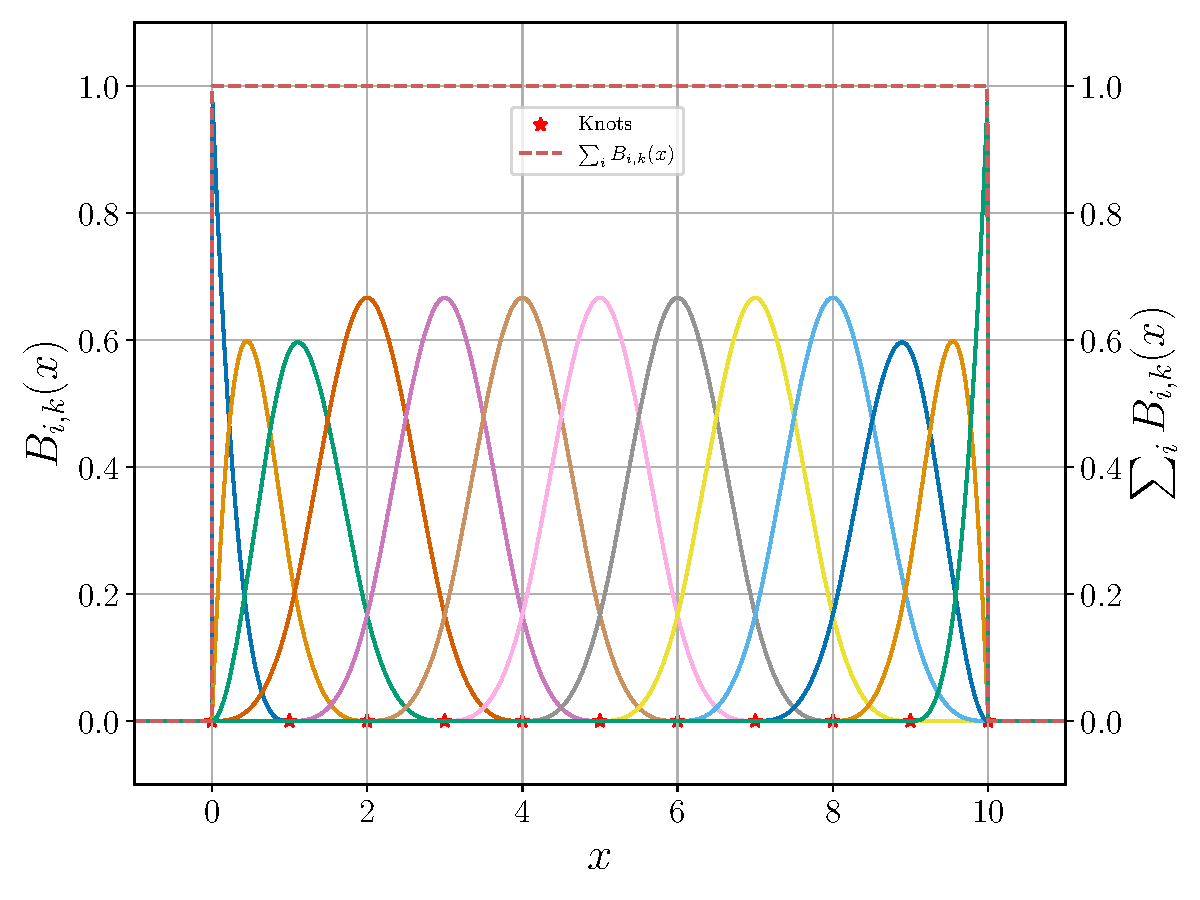
\includegraphics[width=\textwidth]{../plots/B_i_k/B_i.pdf}
        \caption{$B_{i, k=4}$}
        \label{subfig:bik}
    \end{subfigure}
    \begin{subfigure}{0.49\textwidth}
        \centering
        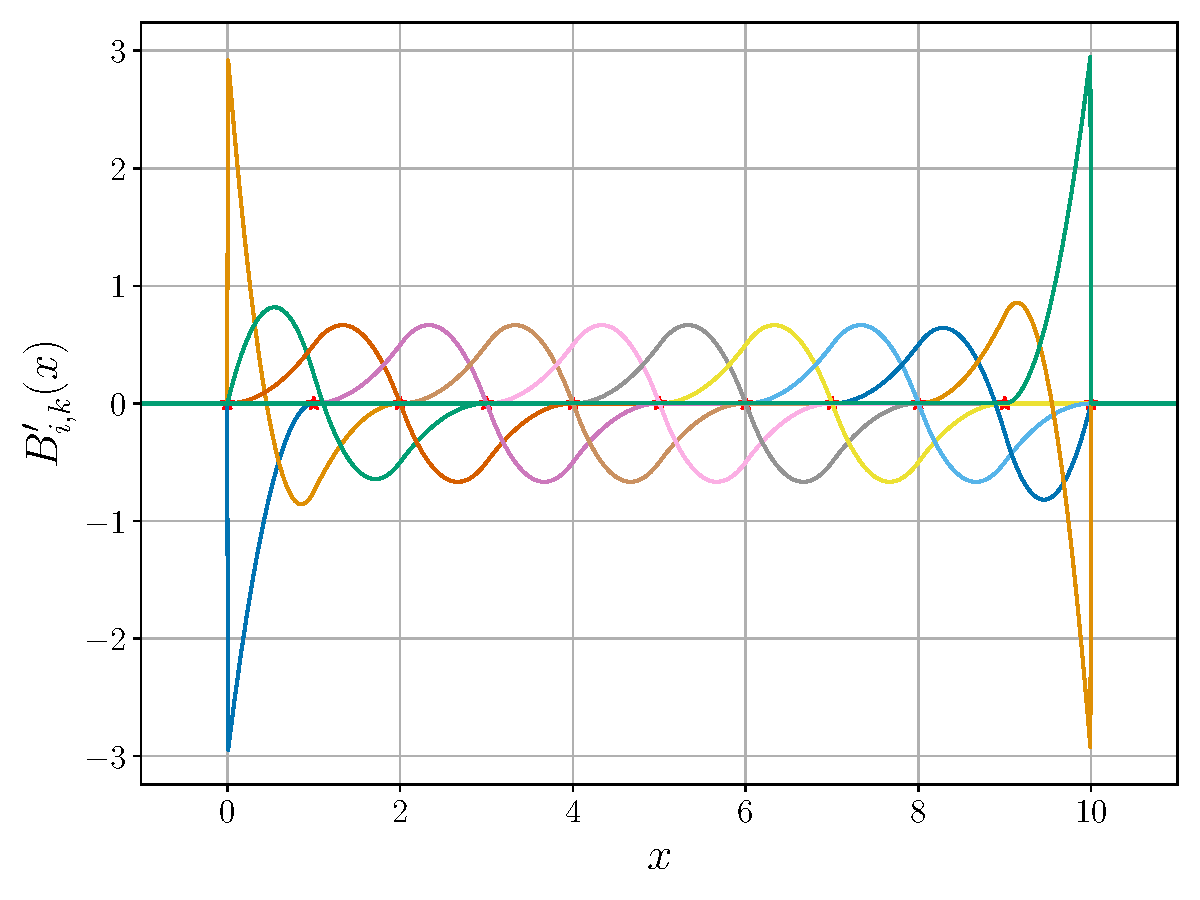
\includegraphics[width=\textwidth]{../plots/B_i_k_x/B_i_x.pdf}
        \caption{$\partial_x B_{i, k=4}$}
        \label{subfig:bik_x}
    \end{subfigure}\\
    \begin{subfigure}{0.49\textwidth}
        \centering
        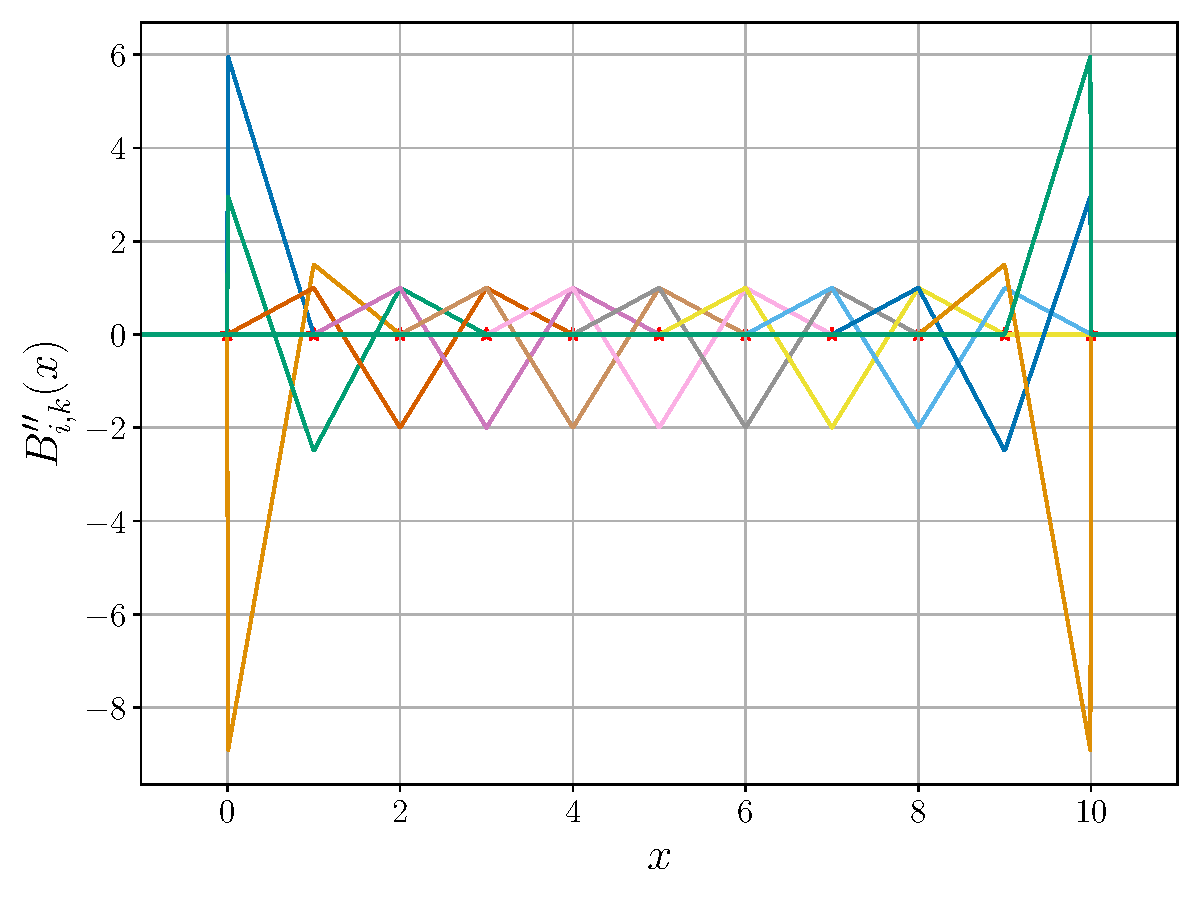
\includegraphics[width=\textwidth]{../plots/B_i_k_xx/B_i_xx.pdf}
        \caption{$\partial_x^2 B_{i, k=4}$}
        \label{subfig:bik_xx}
    \end{subfigure}
    \caption{$k=4$ B-splines on $[0, 10]$ (\ref{subfig:bik}) and their first (\ref{subfig:bik_x}) and second (\ref{subfig:bik_xx}) derivatives with eleven evenly spaced knot points. The splines in \ref{subfig:bik} sum to unity on the entire interval. The first derivative is smooth, while the second derivative is continuous but not differentiable.}
    \label{fig:splines}
\end{figure}

For the three charge densities suggested in the assignment, we present the relative deviation of the numerically obtained potential from the exact result in figure~\ref{fig:errors}. It can be seen that accounting for the discontinuities in $\rho$ is much more important for a good accuracy than using many knot points, see~\ref{subfig:err_sphere},~\ref{subfig:err_shell} as using 12 smartly placed knots vastly outperforms 500 naively placed ones in the case of the solid sphere. 

Furthermore, the exponential charge distribution of hydrogen~\ref{subfig:err_hydro} poses a problem for linearly spaced knots and many are needed for good accuracy. A better approach not explored here might be to use an exponential distribution of points for this charge density.
\begin{figure}
    \centering
    \begin{subfigure}{0.49\textwidth}
        \centering
        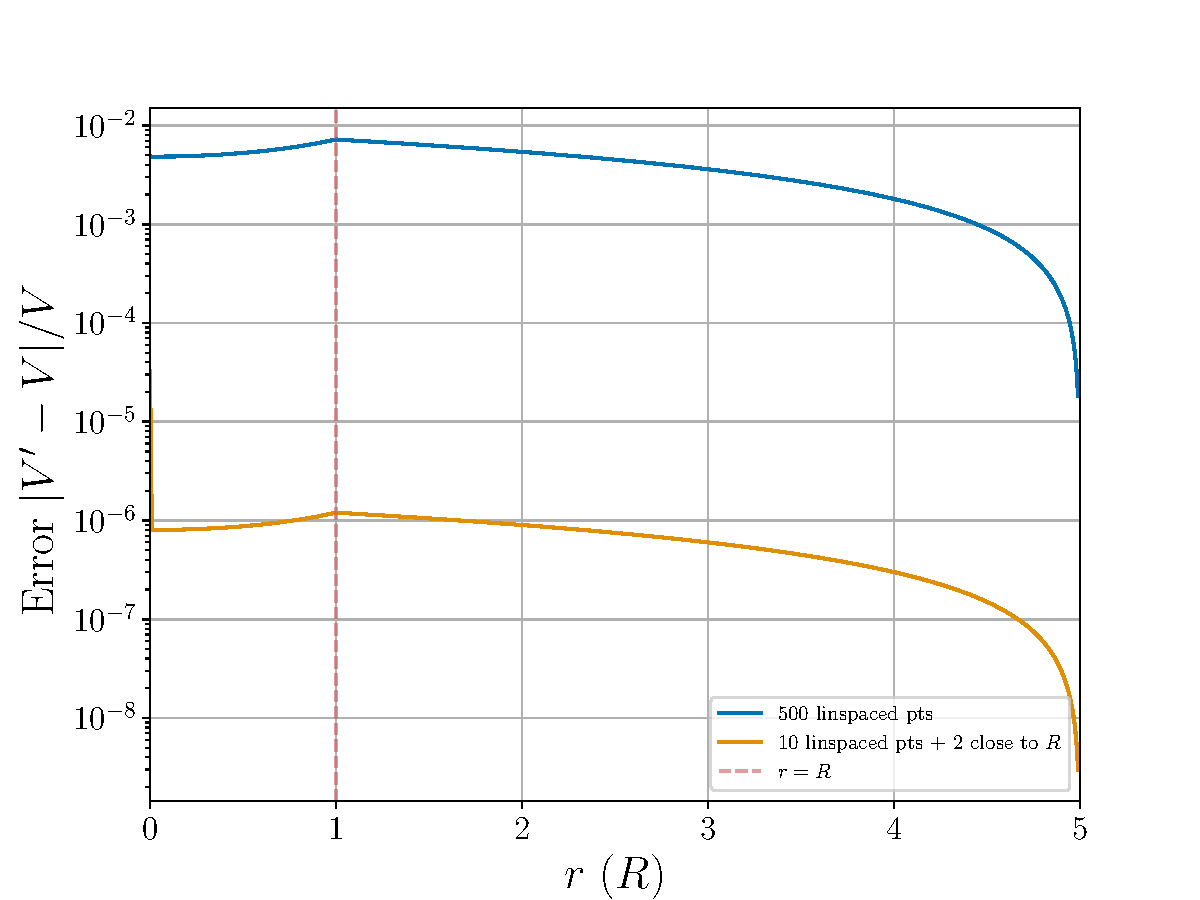
\includegraphics[width=\textwidth]{../plots/potential_error/error_solidsphere_test.pdf}
        \caption{Homogeneously charged sphere}
        \label{subfig:err_sphere}
    \end{subfigure}
    \begin{subfigure}{0.49\textwidth}
        \centering
        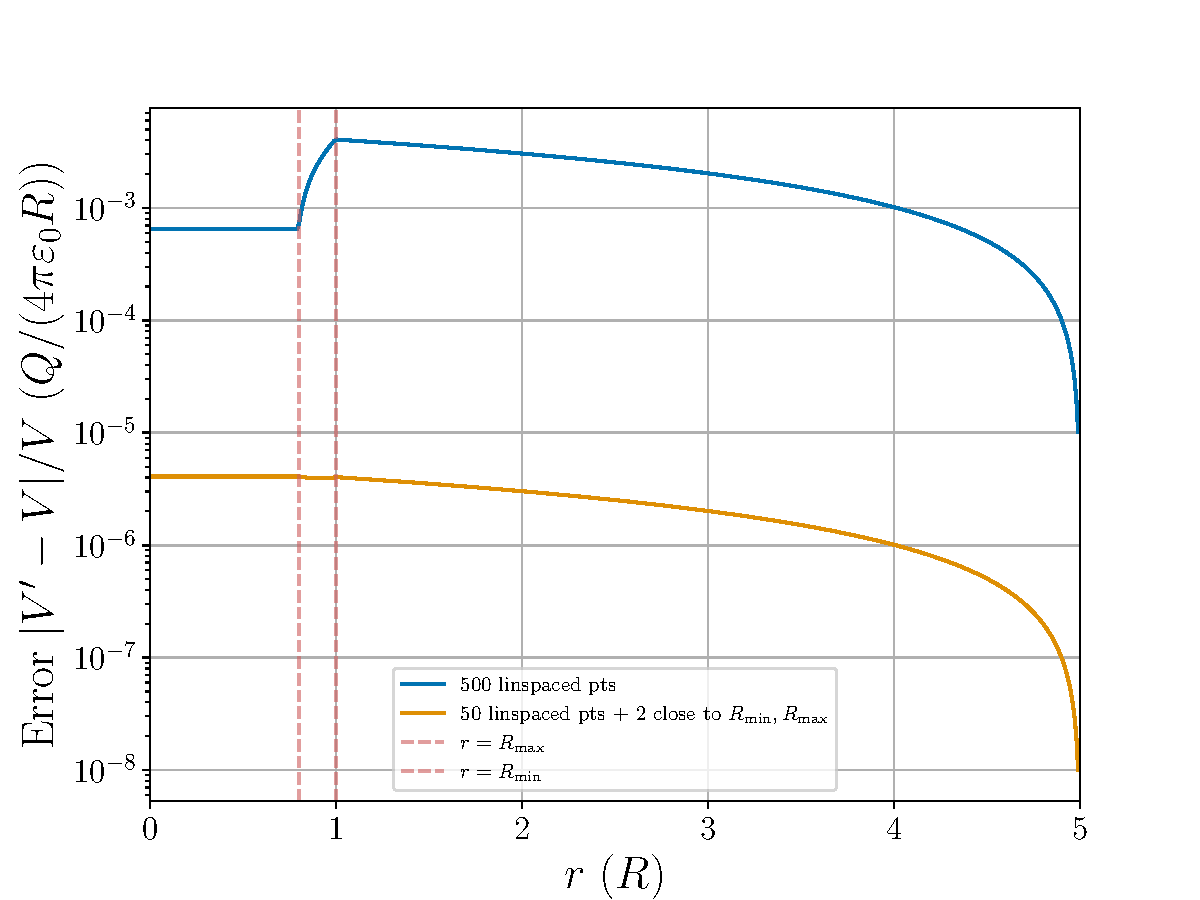
\includegraphics[width=\textwidth]{../plots/potential_error/error_shell_test.pdf}
        \caption{Homogeneously charged spherical shell}
        \label{subfig:err_shell}
    \end{subfigure}\\
    \begin{subfigure}{0.49\textwidth}
        \centering
        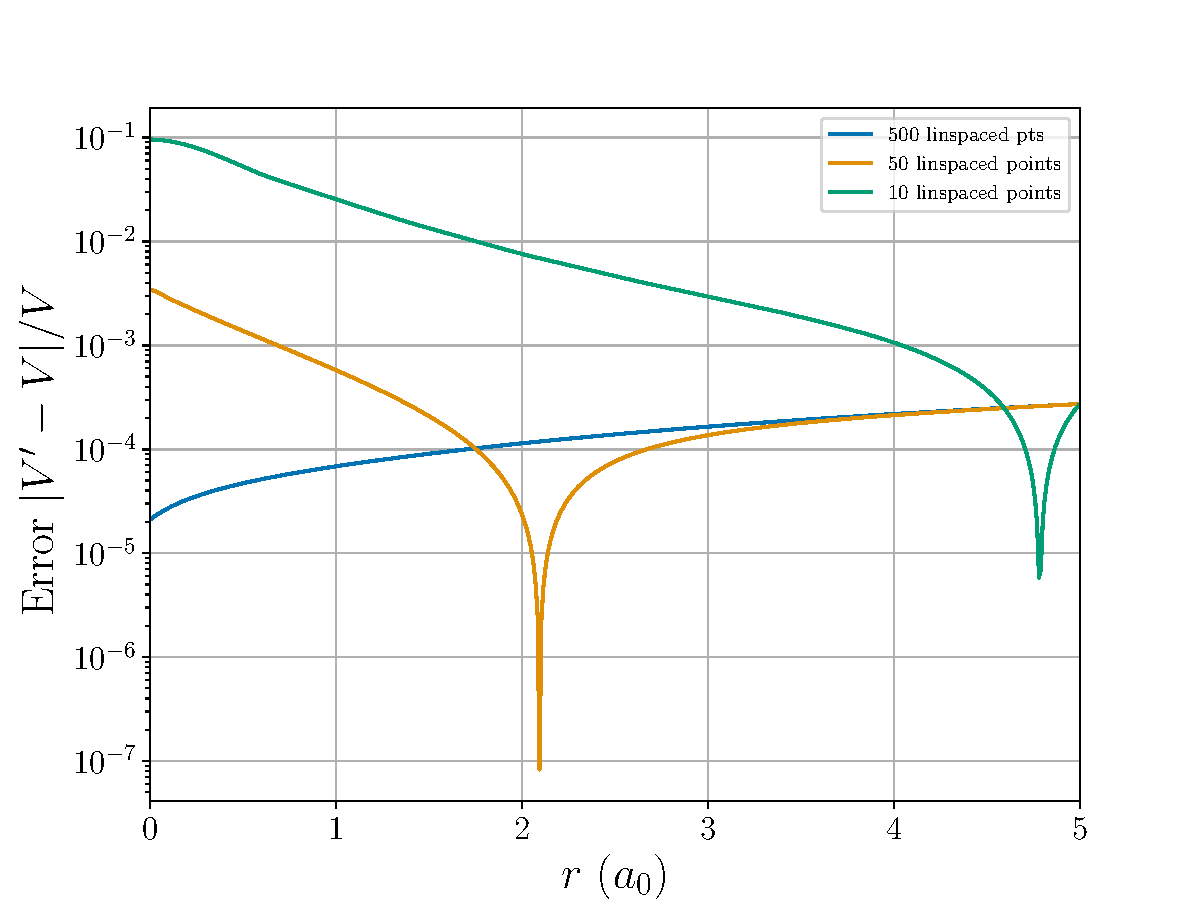
\includegraphics[width=\textwidth]{../plots/potential_error/error_hydrogen_test.pdf}
        \caption{Hydrogen ground state}
        \label{subfig:err_hydro}
    \end{subfigure}
    \caption{Relative error of the numerically obtained potential for different charge densities and different numbers / distributions of knot points. Accounting for the discontinuities in $\rho$ is much more important for a good accuracy than using many knot points, see~\ref{subfig:err_sphere},~\ref{subfig:err_shell}. The exponential charge distribution of hydrogen~\ref{subfig:err_hydro} poses a problem for linearly spaced knots and many are needed for good accuracy.}
    \label{fig:errors}
\end{figure}

\FloatBarrier
\section{Results}
We calculate the potential for the following charge densities and with the following knot point distributions:
\begin{enumerate}
    \item Homogeneously charged sphere:
    \begin{equation}
        \rho(r) = \begin{cases}
            \frac{Q}{V}, & r \leq R \\
            0, & \text{else}
        \end{cases}
    \end{equation}
    10 evenly spaced knot points on $[0, 5R]$ plus two close to the discontinuity at $R\pm1\cdot 10^{-6}R$
    \item Homogeneously charged spherical shell with $R_\text{min} = 4/5\,R_\text{max}$:
    \begin{equation}
        \rho(r) = \begin{cases}
            \frac{Q}{V}, & R_\text{min} \leq r \leq R_\text{max} \\
            0, & \text{else}
        \end{cases}
    \end{equation}
    50 evenly spaced knot points $[0, 5R_\text{max}]$ plus two close to the discontinuities each at $R_\text{min/max}\pm1\cdot 10^{-6}R_\text{max}$
    \item Hydrogen ground state:
    \begin{equation}
        \rho(r) = \frac{e}{\pi a_0^3}\text{e}^{-2r/a_0}
    \end{equation}
    500 evenly spaced knot points on $[0, 5a_0]$
    \item $2s$-state:
    \begin{equation}
        \rho(r) = \frac{e}{32\pi a_0^3}\left(2 - \frac{r}{a_0}\right)\text{e}^{-r/a_0}
    \end{equation}
    1400 evenly spaced knot points on $[0, 14a_0]$
\end{enumerate}
The appropriate boundary conditions for $\varphi(r)$ are $\varphi(0) = 0$ and $\lim_{r\to\infty}\varphi(r)=Q/(4\pi\varepsilon_0 r)$ where $Q=e$ for hydrogen. In our case, $\infty=5R$.

The solutions to Poisson's equation obtained with the collocation method can be seen in~\ref{fig:pot}. For the first three, the exact solutions are also shown, and we observe good to excellent agreement.

The potential for the $2s$-state of Hydrogen shows a bend at $r=2a_0$ where the charge density vanished, which appears reasonable.
\begin{figure}
    \centering
    \begin{subfigure}{0.49\textwidth}
        \centering
        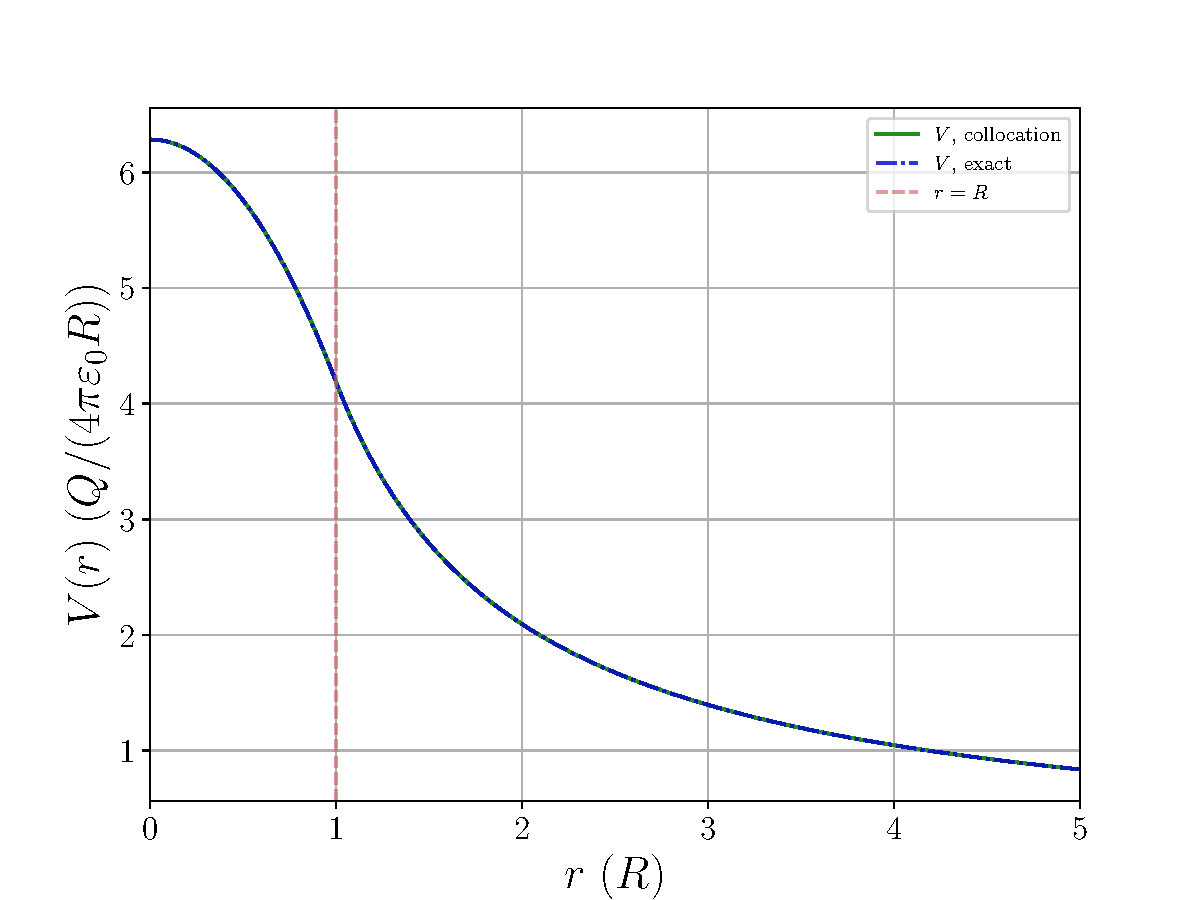
\includegraphics[width=\textwidth]{../plots/potential/potential_solidsphere_test.pdf}
        \caption{Homogeneously charged sphere}
        \label{subfig:sph}
    \end{subfigure}
    \begin{subfigure}{0.49\textwidth}
        \centering
        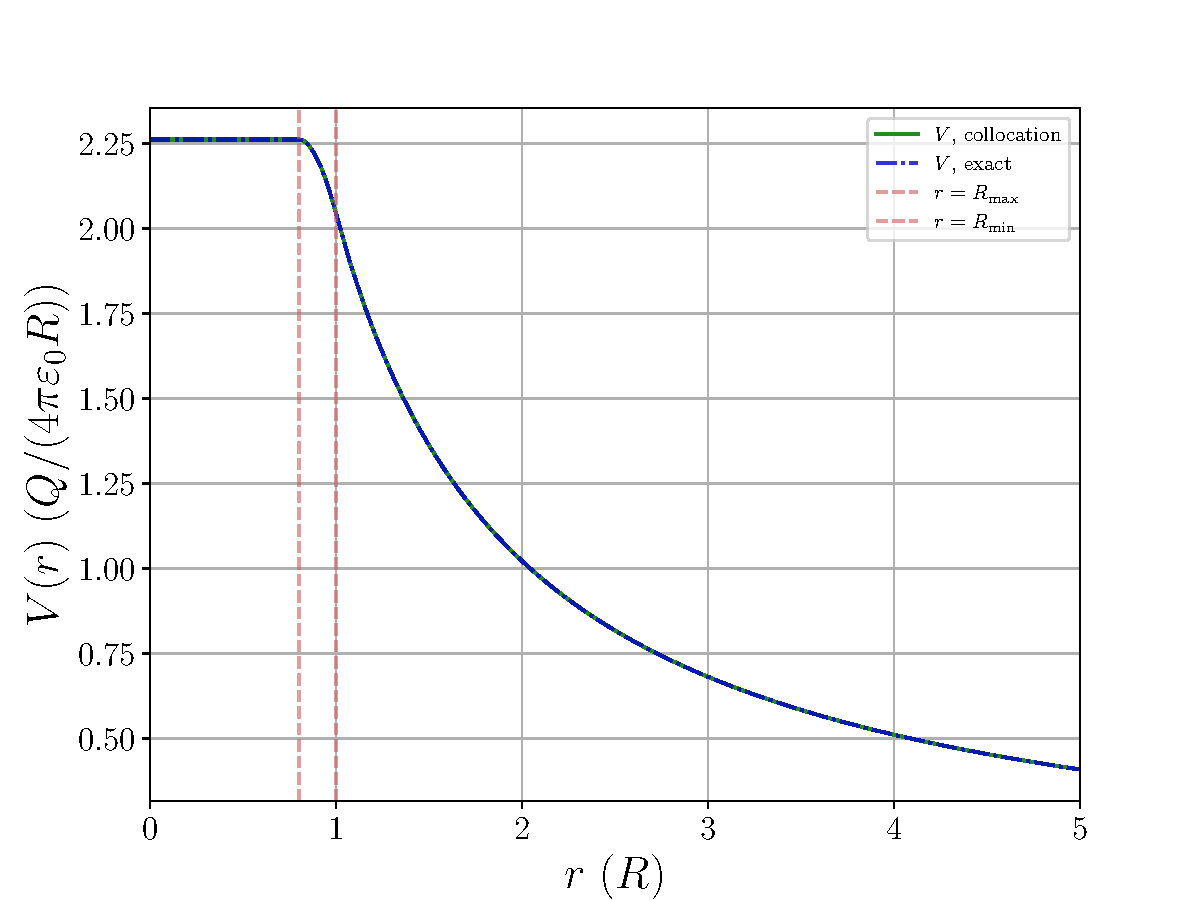
\includegraphics[width=\textwidth]{../plots/potential/potential_shell_test.pdf}
        \caption{Homogeneously charged spherical shell}
        \label{subfig:shell}
    \end{subfigure}\\
    \begin{subfigure}{0.49\textwidth}
        \centering
        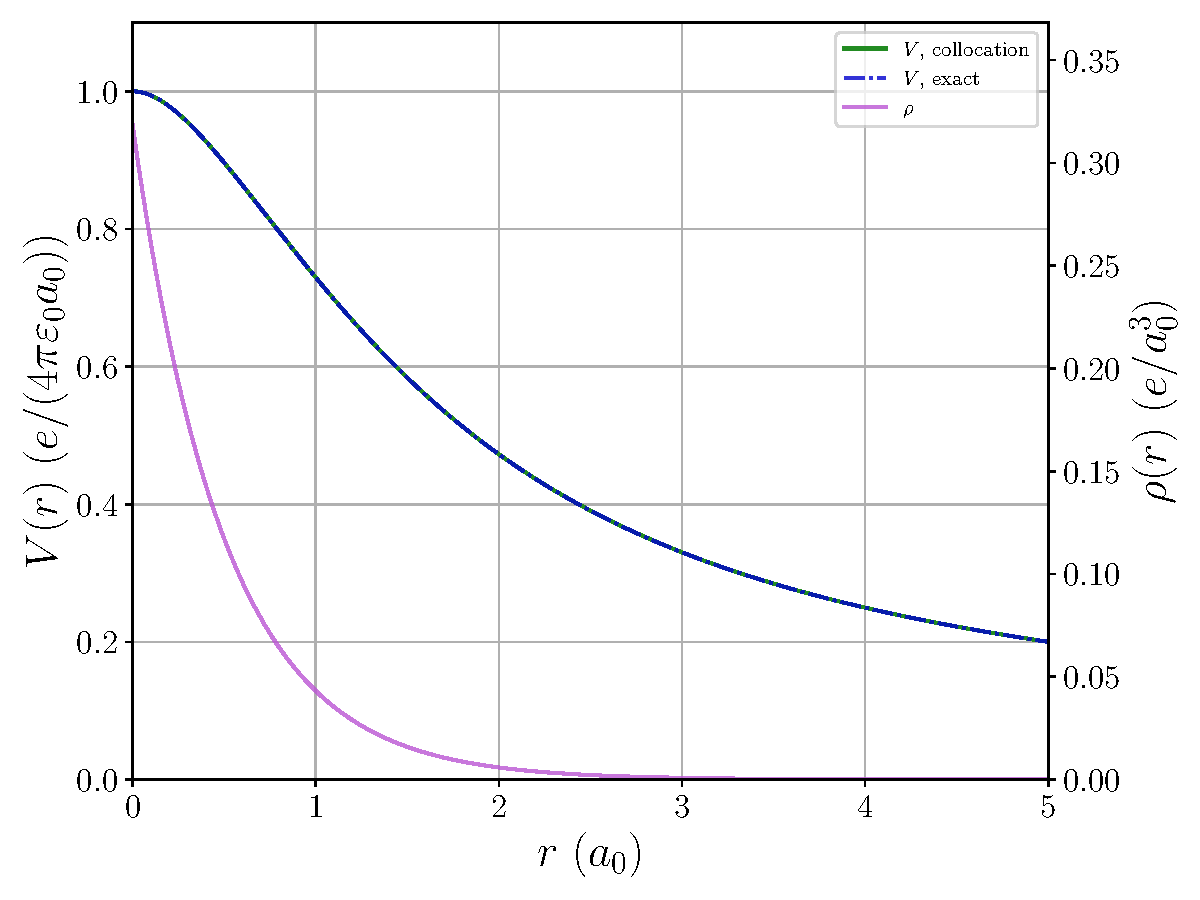
\includegraphics[width=\textwidth]{../plots/potential/potential_hydrogen.pdf}
        \caption{Hydrogen $1s$-state}
        \label{subfig:hydro}
    \end{subfigure}
    \begin{subfigure}{0.49\textwidth}
        \centering
        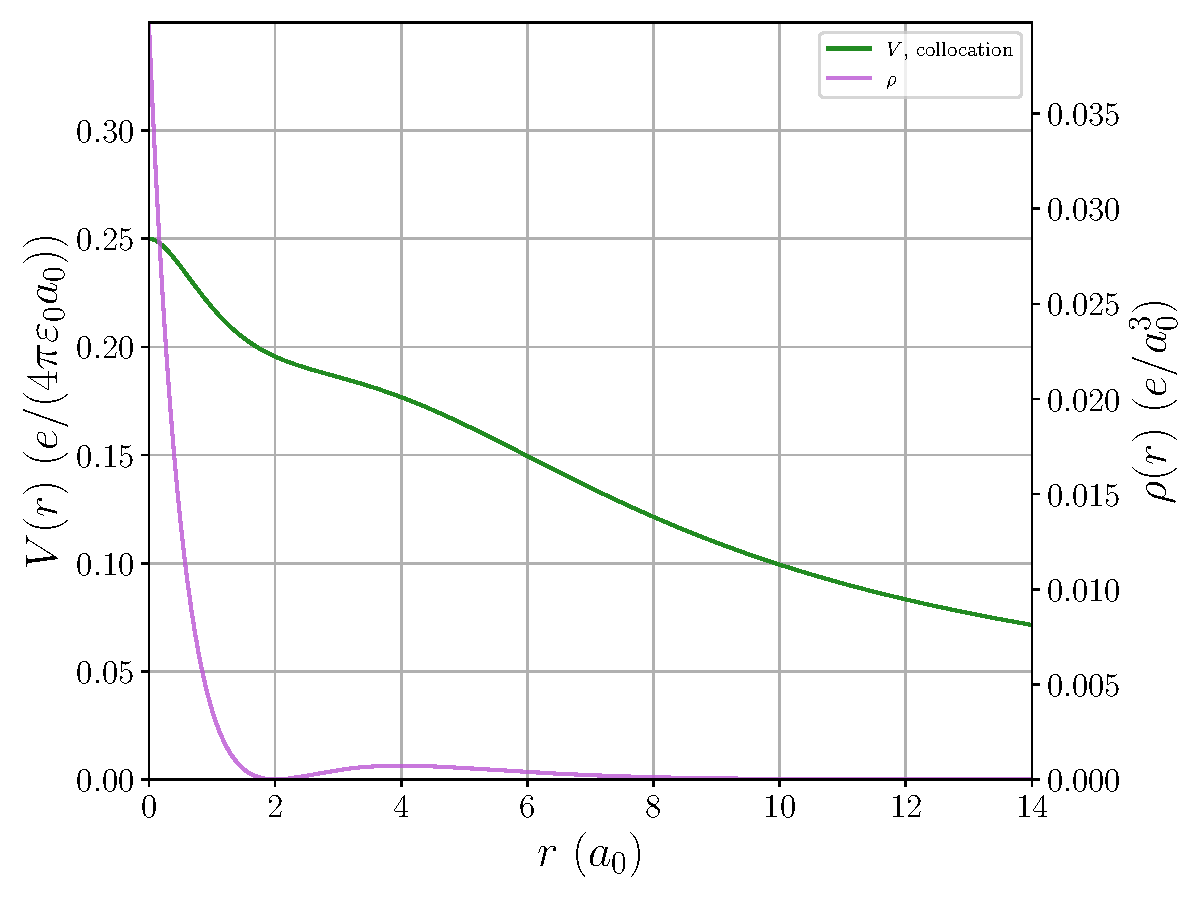
\includegraphics[width=\textwidth]{../plots/potential/potential_hydrogen_2s.pdf}
        \caption{Hydrogen $2s$-state}
        \label{subfig:hydros2}
    \end{subfigure}
    \caption{Numerically obtained electrostatic potentials for different charge densities.}
    \label{fig:pot}
\end{figure}

\FloatBarrier
\section{Conclusion}
We have successfully implemented B-splines and the collocation method in a high-level language and applied it to Poisson's equation, achieving good results in comparison to the exact solutions.

\newpage
\FloatBarrier
\fakesection{References}
\printbibliography


\end{document}
